\documentclass{article}

\usepackage{amsfonts} % for "\mathbb" macro
\usepackage{enumerate}
\usepackage{graphicx}
\usepackage{hyperref}
\usepackage[shortlabels]{enumitem}
\usepackage{makecell}
\usepackage{subcaption}
\usepackage{svg}
\usepackage{tabularx}
\usepackage[disable]{todonotes}
%\usepackage{todonotes}
\usepackage{url}

\title{Procedural generation of fixed-viewpoint digital nature landscapes.}
\author{Lars van Arkel}

\begin{document}

\maketitle

\section{Introduction}
Procedural Content Generation (PCG) has been actively researched in computer graphics for years. For developers generating virtual content can become time-intensive, and PCG has been used to reduce the workload of creating virtual terrains. One important aspect is the trade-off between the control the user has over the generated terrain against the amount of effort required to create the terrain. For this research, we will be designing a system to generate complete landscapes which will be rendered from ground level. Besides combining multiple features, this research will aim to give a qualitative evaluation of the generated terrain with rules that can be specified by the designer. This system will then be used to create landscapes as part of the Growing Roots research project.
\todo{Show how this system will be different than other implementations.}

\section{Problem statement}
As part of the Growing Roots research project\footnote{Growing Roots. From \url{https://growingroots.nl}, retrieved at 16-11-2024}, a device called the ``virtual window" is developed by the company TexTown Games\footnote{Design2Connect - TexTown Games. From \url{https://textowngames.nl/portfolio/design2connect/}, retrieved at 10-1-2025}. This device tracks the position of a person in front of a monitor and projects a landscape on the screen based on where the person is standing. Currently, only handcrafted landscapes are used for testing the system. For further research related to emotional impressions of landscapes, more environments are needed that differ in visually distinguishable parameters, such as the density of trees or the color and types of vegetation used. Handcrafting landscapes takes a significant amount of time, so the ability to create more terrains automatically is required. The landscapes generated will be landscapes of nature, with some man-made structures such as roads or benches. 

The generated terrain will only be used for the virtual window, which means that the camera will not move around the landscape. This limits the size and amount of terrain that needs to be generated. Therefore, each feature's order and properties will be generated with this rule in consideration.

Research in procedural terrain generation has often focused on generating large-scale terrain, but the virtual window only allows a smaller view on the terrain. This results in the generated terrain having a larger focus on smaller details such as vegetation and visible parts of the terrain.

As further research will focus on the effect of different terrain features, the researcher needs control over the terrain they want to create. This control should allow the user to select broader features of the terrain, such as the kind of ecology the terrain represents, and finer features, such as the density of vegetation or ruggedness of the ground.

As the system will be used by people who are not necessarily designers or programmers, the generation of the terrain will be automated with little user input. Because of this, we must be able to verify whether the generated terrain adheres to required constraints. These features can be broad for the entire terrain, such as that some desired biomes are included, or specific to the point of view, such that a large part of the generated is visible from the viewpoint.

\section{Research questions}
\begin{enumerate}[label={RQ \arabic*:}]
    \item How can we generate each component in a landscape, and how do these components work together and interact to create a landscape suited for a single point of view?
    \begin{enumerate}[label={RQ 1.\arabic*:}]
        \item What components are required to generate a landscape?
        \item How can we generate each component required for the landscape?
        \item How can we connect all components to create a landscape for a single point of view?
    \end{enumerate}

    \item How can we parameterise each component to create distinctive environments, while the effect of each parameter is clear?
    \begin{enumerate}[label={RQ 2.\arabic*:}]
        \item How do we define different environments to be distinctive?
        \item How can we use parameters to distinguish between different environments?
    \end{enumerate}

    \item In what ways can we validate the procedurally generated terrain?
    \begin{enumerate}[label={RQ 3.\arabic*:}]
        \item How can different requirements be translated into rules to validate the terrain?
        \item How can the terrain generation be influenced by the validation to create terrain conforming to certain rules?
    \end{enumerate}
\end{enumerate}

\input{chapters/background}

\section{Architecture}
To create digital environments, we have created a framework that generated procedural natural environments consisting of surface terrain, rivers and vegetation objects using pre-generated assets. For each component of the system, different parameters are used to influence the system such that a desired environment is generated. The system is designed to be modular when generating the different components, and is configurable to skip the generation of some components when it is not necessary to generate. \todo{Maybe write a bit more about how to use the system.}
% The architecture of the system consists of different components which are then combined.
% In this section, explain the architecture of the system.
% Show how the different components of the system interact, and what data is stored in each step
% Show how the chunk system is used to segment the generation.
% Explain that for mesh sizes and supporting a larger world, the terrain is split up into chunks.

\subsection{Generating components}
% Introduce the different components, and describe that each component has different parameters that are described in each section
The proposed system consists of three different components. The first is the terrain. This terrain forms the basis of the landscape on which different features can be placed. The second component consists of water features. These water features, which consist of rivers and ponds, are generated based on a number of control points which are placed onto the terrain. Thirdly, the last component of the system is the placement of vegetation. Vegetation consists of different type of plants, ranging from small bushes to large trees. The generation of each component can be described with a number of parameters. While some parameters would be dependent on the initial settings of the terrain, others can wildly influence the type of landscape created.

In this subsection, the generation of the different components is described in isolation from each other, as well as the parameters required for each component. For each parameter, a description is given what the parameter does in the generation of the component, and how the system can interact with the parameter.

\subsubsection{Terrain}
% Describe what algorithm is chosen and why
In our design, we have chosen to generate terrain using Fractal noise using Perlin noise \cite{musgrave_synthesis_1989}. The advantage of using noise functions is that the calculation of each separate point can be performed in parallel. Each chunk can be generated independent of other chunks.
% Describe the alternative Diamond Square method, and why it does not work correctly with the chunk system
The main downside of using the previously mentioned midpoint displacement algorithm in our architecture is in the chunk system. When generating a chunk with midpoint displacement, the vertices depend on their neighbours and a random offset. In different chunks, these offsets do not correspond to the same values, resulting in different height values for vertices along the edges of neighbouring chunks. To solve this, the height values of vertices can be calculated using the different chunks, but this creates a dependency between chunks.

% Show how the terrain is generated
The terrain is generated on a 2D grid of vertices. For each octave, a separate random 2D offset is generated to be used in the Perlin noise function. This offset is scaled and translated by the scale and position of the vertex in the grid. These coordinates are evaluated using Perlin noise and scaled by the amplitude. The sum of these values is the resulting value in the height map.
To properly overlap different chunks, the last value of each heightmap is scaled to use the same coordinates as the first value of the neighbouring chunk.

% Describe the parameters of the system, and how they are used to create the heightmap.
The parameters that influence the algorithm are shown in table \ref{tab:perlin-parameters}. In this table we make a distinction between parameters that are set by the system because they are constant or implicit based on other systems such as the chunk system, and parameters that can be influenced by a designer.
The width and depth of the system will be fixed, since the amount of vertices in a chunk is deemed to be constant. The offset and seed are implicit in the execution of the program, since the offset is defined by which chunk will be generated and the seed is constant per generation of the system, to provide the same base noise offsets for all chunks.

\begin{table}[ht]
\begin{tabularx}{\linewidth}{|l|l|l|X|}
\hline
Name & Type & Bounds & Description\\
\hline
Width & Int & $\geq 1$ & The width of the heightmap in vertices\\

Height & Int & $\geq 1$ & The depth of the heightmap in vertices\\

Offset & Vec2Int & $\mathbb{Z}^2$ & The chunk coordinates of the generating chunk\\

Seed & Int & $\mathbb{Z}$ & The seed that initialises the random number generator\\

\hline

Scale & Float & $> 0$ & The initial frequency of the noise on the terrain\\

Octaves & Int & $\geq 1$ & How many iterations of the fractal function is applied\\

Persistance & Float & $\geq 0$ & How much the amplitude of the noise is reduced multiplicatively each octave \\

Lacunarity & Float & $\geq 0$ & How much the frequency of the noise is increased multiplicatively each octave \\
\hline

\end{tabularx}
\caption{The parameters used in the fractal noise algorithm. The top section contains constant or implicit parameters, the lower part contains parameters used by the designer.}
\label{tab:perlin-parameters}
\end{table}

% Parameter analysis

% Texturing (Still to be implemented)

\subsubsection{Rivers and ponds}
% The generation of rivers and ponds consist of 2 separate tasks.
The generation of rivers and ponds consist of 2 separate tasks. The first step is to plan the route or shape of the river. After that, the path can be combined with a profile to generate the water.
% First the path of the river needs to be established. This is done by placing points.
% These points form a curve that is used to, together with a curve profile, generate a fat mesh that can be added to the curve.
When the path of the river has been defined, a bezier curve is plotted through the points. When a pond is generated, the end of the curve is connected to the start. Like the system proposed by Huijser\cite{huijser_procedural_2010}, the curve is transformed into a mesh, the fat curve, that can be used in other stages of the program. To transform the path of a river to a fat curve, each curve point is given a width with which a line is constructed perpendicular to the curve. The line creates a triangle mesh with triangles between the curve points. When generating a pond, the middle of the curve is established by taking the average position of all points. The triangles of the mesh are defined by the middle of the curve and two subsequent curve points. Using this fat curve we can check whether a point is inside or outside the curve, and by calculating the barycentric coordinates of a point, the location of that point in the cross-section of the curve is derived. This coordinate can be used with the profile to derive the depth of the river at that location.

% Parameters of path planning

% Parameters of fat curve creation
The parameters that describe the creation of the fat curve are shown in Table \ref{tab:river-fatcurve-parameters}

% Parameter table fatcurve
\begin{table}[ht]
\begin{tabularx}{\linewidth}{|l|l|l|X|}
\hline
Name & Type & Bounds & Description\\
\hline

tangentLength & float & $\mathbb{R}$ & How far the tangents of the bezier curve are scaled. \\

CurvePoint.Direction & Vec3 & $\mathbb{R}^3$ & For each point, the gradient along the curve\\

MeshSubdivisions & int & $\geq 0$ & How many points are interpolated between curvePoints\\

\hline

CurvePoint.Position & Vec3 & $\mathbb{R}^3$ & For each point in the curve, the position in the world\\

CurvePoint.width & float & $> 0$ & For each point, the width of the river along the point\\

closed & boolean & T/F & Whether the curve describes a river (F) or a pond (T) \\
\hline

\end{tabularx}
\caption{The parameters used for generating a fat curve}
\label{tab:river-fatcurve-parameters}
\end{table}

\subsubsection{Placing vegetation}
% Placing vegetation has to adhere to a few rules
In the system, we introduce two different types of placing vegetation. The first method uses the Poisson Disk Distribution to generate points that have a minimum distance from each other. To generate the points, the paper of Bridson \cite{bridson_fast_2007} is used. We have expanded this initial algorithm so that it is able to be used with multiple types of points, where each type of point has a different minimal distance. This approach can be used to generate multiple different types of vegetation.

To generate different types of vegetation, we separate the types of vegetation into different layers, similar to the solution provided by do Nascimento et al. \cite{do_nascimento_gpu-based_2018}. For each separate layer, points are randomly generated. Based on the paper of Bridson, we use a 2-dimensional grid to store the points, with the size of each grid cell being equal to $d / \sqrt{2}$, where $d$ is the minimum distance of two points, which is twice the radius of the object on the layer. Given a boundary where the points lie, the algorithm places points around already generated points until there is no point that can be the neighbour of a new point.

The parameters that describe the placement of points on a single layer are shown in table \ref{tab:pdd-single-layer}. The retries parameter is constant, and a value of 30 is typically used.\\

% Parameter table single-layer PDD
\begin{table}[ht]
\begin{tabularx}{\linewidth}{|l|l|l|X|}
\hline
Name & Type & Bounds & Description\\
\hline

bounds & AABB & Area > 0 & The area wherein objects can be placed. \\
\hline

radius & float & $> 0$ & The radius of an object, or half the minimum distance between points. \\

\hline

retries & int & $\geq 0$ & How many times an already generated point tries to generate an adjacent point until it fails. \\
\hline

\end{tabularx}
\caption{The parameters used for generating a PDD layer}
\label{tab:pdd-single-layer}
\end{table}

To combine multiple layers generated by the PDD, we generate all layers from large to small, and when each layer is generated, all points are filtered by checking if there is overlap with a larger layer. In our system, we can assign a different radius for objects in the same layer as objects in a lower layer. The justification for this is as follows: When placing trees in an environment, their canopies cannot overlap but smaller objects, such as bushes, can be placed within the radius of the canopy but are still blocked by the size of the trunk.

As different layers have different radii, their 2-dimensional grid structure have different sizes. While in the single layer algorithm we only had to check the 8 neighbours of a cell, the size of the neighbourhood differs when different sized grids are used. The radius of the neighbourhood equals $\lceil (r_1 + r_2) / cell\_size_1 \rceil$, with $r_1, cell\_size_1$ corresponding to the larger layer and $r_2$ being the radius of the smaller layer.

The parameters used in the Multi-layer PDD algorithm are shown in table \ref{tab:pdd-multi-layer}. For each layer of the input, the algorithm returns the positions that do not overlap with higher layers.

% Parameter table Multi-layer PDD
\begin{table}[ht]
\begin{tabularx}{\linewidth}{|l|l|l|X|}
\hline
Name & Type & Bounds & Description\\
\hline

bounds & AABB & Area $> 0$ & The area wherein objects can be placed.\\
\hline

layers & Layer[] & size $> 0$ & The different layers of object used in the algorithm.\\
\hline

Layer.layerRadius & float & $> 0$ & The radius of the object within the same layer.\\
\hline

Layer.innerRadius & float & $> 0$ & The radius of the object when checking lower layers.\\
\hline

retries & int & $\geq 0$ & How many times an already generated point tries to generate an adjacent point until it fails. \\
\hline

\end{tabularx}
\caption{The parameters used for generating multiple PDD layers}
\label{tab:pdd-multi-layer}
\end{table}

Our second approach follows the method proposed by Lane et al. \cite{lane_generating_2002}, which uses a probability density function to randomly place objects. Each object placed modifies the probability function with a kernel which has a circular influence on the probability function. The kernel is defined by a radius and a curve, where the value of the curve is equal to the ratio that the probability function will change. Examples of kernels are shown in Figure \ref{fig:deformation_kernel_example}. When using kernel C from this example, new objects have a lower probability to be placed near other objects. Alternatively, using kernel A increases the probability of a new object being placed close to another object.

\begin{figure}
    \centering
    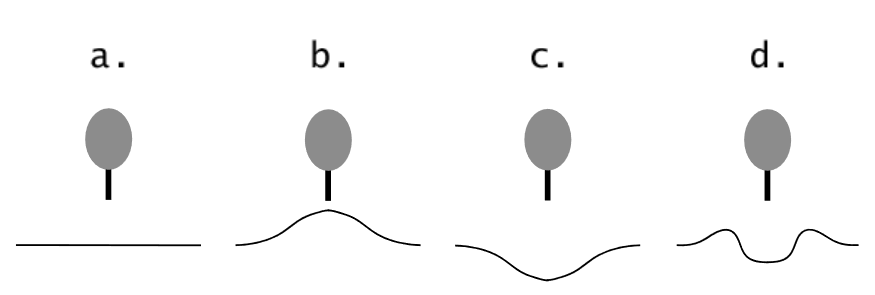
\includegraphics[width=0.9\linewidth]{figures/deformation_kernel_example.png}
    \caption{Examples of kernels that can be used in the deformation kernel algorithm, from \cite{lane_generating_2002}.}
    \label{fig:deformation_kernel_example}
\end{figure}

\todo{Fix formatting of table}
% Parameter table Deformation kernel
\begin{table}[ht]
\begin{tabularx}{\linewidth}{|l|l|l|X|}
\hline
Name & Type & Bounds & Description\\
\hline

bounds & AABB & Area $> 0$ & The area wherein objects can be placed.\\
\hline

deformationObject & DeformationKernel & & The deformation kernel used in updating the density function.\\
\hline

DeformationKernel.curve & AnimationCurve & $f(x) \in [0, 1]$ & The function that is used to deform the probability density function.\\
\hline

DeformationKernel.radius & float & $> 0$ & The size of the influence of the deformation kernel.\\
\hline

iterations & int & $\geq 0$ & The amount of objects to be placed.\\
\hline

fieldSize & int & $> 0$ & The size of the array used as probability density function.\\
\hline

\end{tabularx}
\caption{The parameters used for placing objects with a deformation kernel}
\label{tab:deformation-kernel}
\end{table}

\todo{Table for deformation kernel parameters}

% Elaborate PDD and explain second algorithm

% - Vegetation can be separated into a few different layers, representing different kinds of plants (trees, bushes and grass)\

% - Each piece of vegetation has to be placed a minimum distance apart from each other plant.

% - Vegetation from different layers should not overlap

% - The distance of a plant on layer X is not necessarily equal to the distance of layer Y (e.g. canopy of trees exists on tree layer, but on lower layers the trunk of the tree applies.

% Multilevel PDD placement

% Deformation kernel


\subsection{Connecting components}
% Describe the architecture of how the different components combine

\subsubsection{River path planning}
% TODO: Find a way to path a river

\subsubsection{Vegetation selection}
% TODO: Find a way to select vegetation



\section{Parameter analysis}
% Introduce the analysis of the different parameters, and show that in this chapter we will see how changing each parameter can influence different parts of the system.

% Terrain generation
% Show how the different parameters of noise generation influence the resulting heightmap

% Curve planner
% Background already discusses the parameters. Compare this with own experiments

% Pdd generator
% show the impact of radius and density.
\subsection{Pdd placement and object density}
In the PDD placement algorithm the placement of the objects is dependent on the radius of each layer. Changing the radius of an object changes the minimum distance between two objects. The density of the objects placed can therefore be changed by increasing the radius. To show the effect of the radius on the density, we take an initial radius $r$ that represents the bounds of the object itself. We increase this radius by a factor $f$ and run the algorithm. From the amount of points placed we calculate the area that the points occupy with the original radius, and calculate the density. To see the effect of increasing the radius of an object, we take a range from 1 to 4, with increments of 0.2. For each ratio, we run the algorithm 500 times, and calculate the density by calculating the circular area of the initial radius. The results of this example are shown in figure \ref{fig:pdd-parameters-example}, along with a few examples showing the change of radius. The blue bars show the results of the experiment, and the orange line is an exponential distribution, fitted on the data. From this we can see that the density generally follows an exponential distribution. In the examples we can see that increasing the layer radius reduces the places that objects can be placed. % Should probably write more.


\begin{figure}
    \begin{subfigure}{.5\textwidth}
        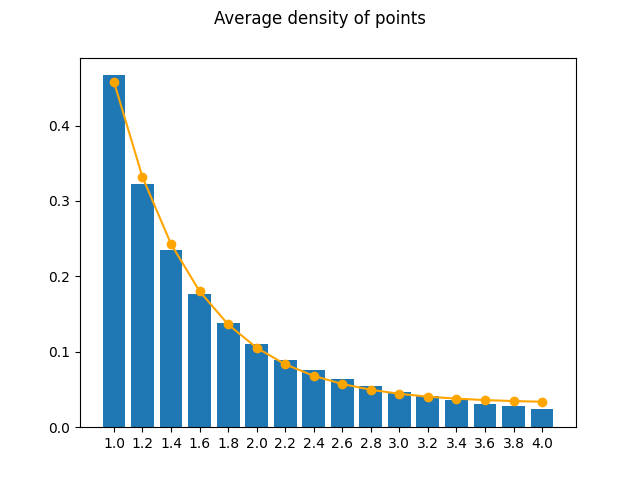
\includegraphics[width=\linewidth]{figures/parameters/pdd-parameters-graph.png}
    \end{subfigure}
    \begin{subfigure}{.5\textwidth}
        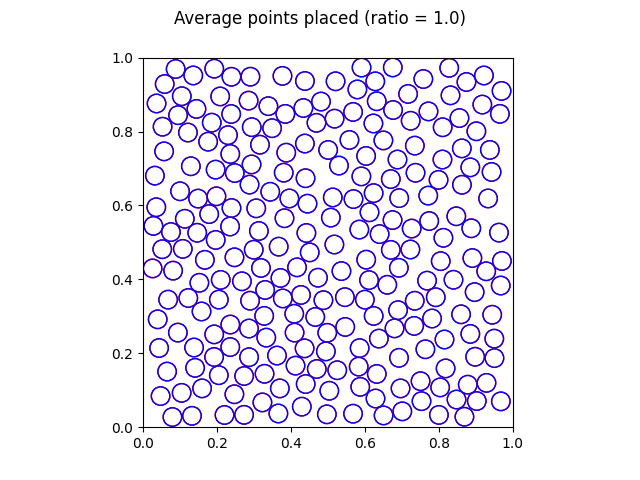
\includegraphics[width=\linewidth]{figures/parameters/pdd-parameters-example-1.png}
    \end{subfigure}
    \begin{subfigure}{.5\textwidth}
        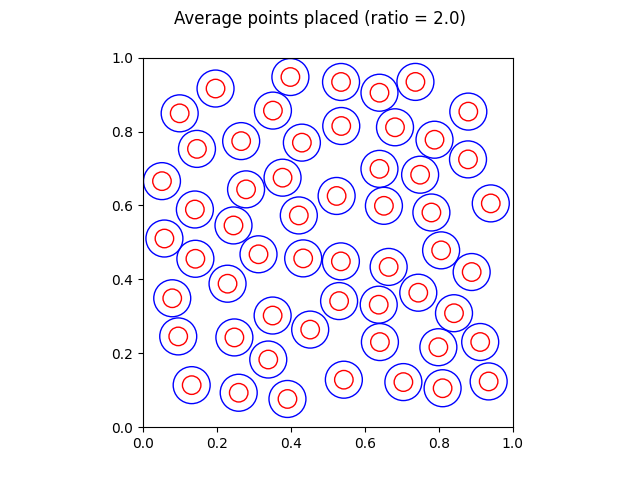
\includegraphics[width=\linewidth]{figures/parameters/pdd-parameters-example-2.png}
    \end{subfigure}
    \begin{subfigure}{.5\textwidth}
        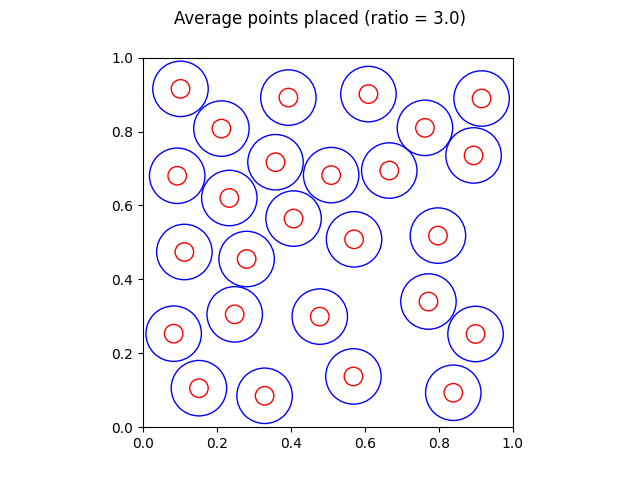
\includegraphics[width=\linewidth]{figures/parameters/pdd-parameters-example-3.png}
    \end{subfigure}
    \caption{Graph of the influence of radius on density, and examples of increasing the radius (blue) on an initial radius (red)}
    \label{fig:pdd-parameters-example}
\end{figure}



\section{Validation}
% Discuss different ways of validating the terrain.
% Describe what we want, and why we want this
    % See rivers from the fixed-point

\subsection{Object segmentation}
When validating the terrain, we want to make a distinction between different types of objects, such as the difference between the ground and rivers, or between the sky and placement objects. To solve this we use object segmentation, which is regularly used in computer vision \cite{kirillov_panoptic_2019}. In object segmentation we make a distinction between semantic segmentation, where all objects of the same type have the same colour, and panoptic segmentation, where each object has a different colour, regardless of it's type.

In our implementation we use a custom shader to colour the individual objects. When analysing the resulting image, we use pixel counting to find the relative size of the object in the view.

An example of applying image segmentation on a landscape is shown in figure \ref{fig:segmentation}. In this image we can see the original landscape on the top-left, and the segmented images on the right. The top image shows the object segmentation where the different kinds of placement object have a shared colour. The bottom image shows panoptic segmentation, where each object has an individual colour.

\begin{figure}
    \begin{subfigure}{.5\textwidth}
        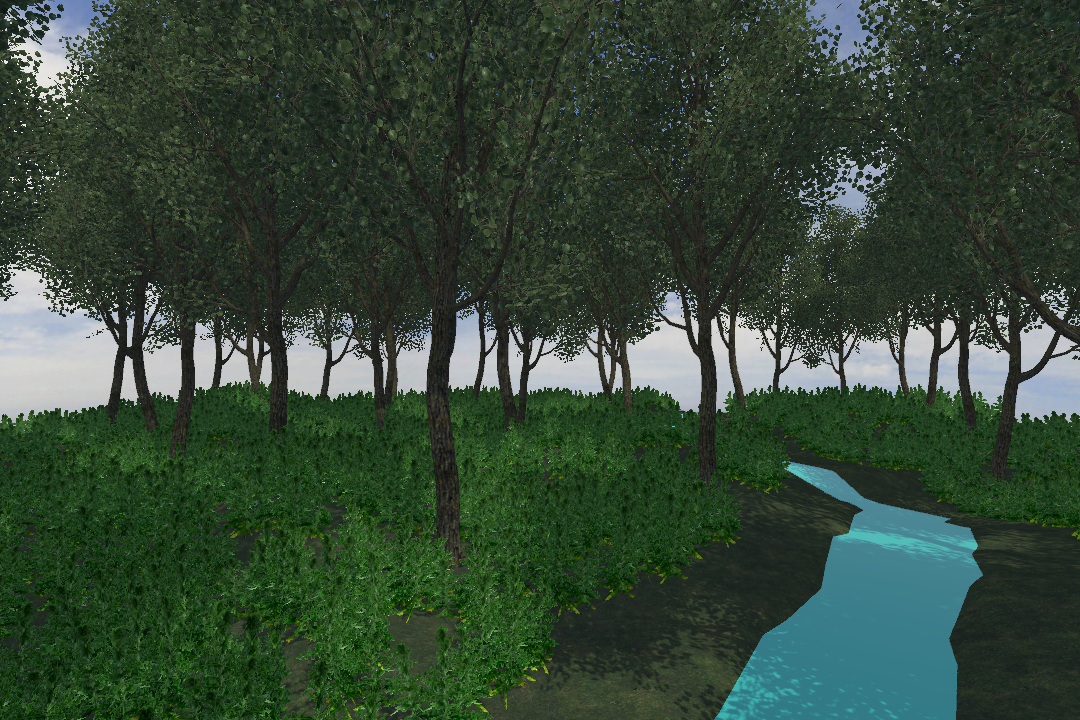
\includegraphics[width=\linewidth]{figures/validation/world_regular.png}
    \end{subfigure}
    \begin{subfigure}{.5\textwidth}
        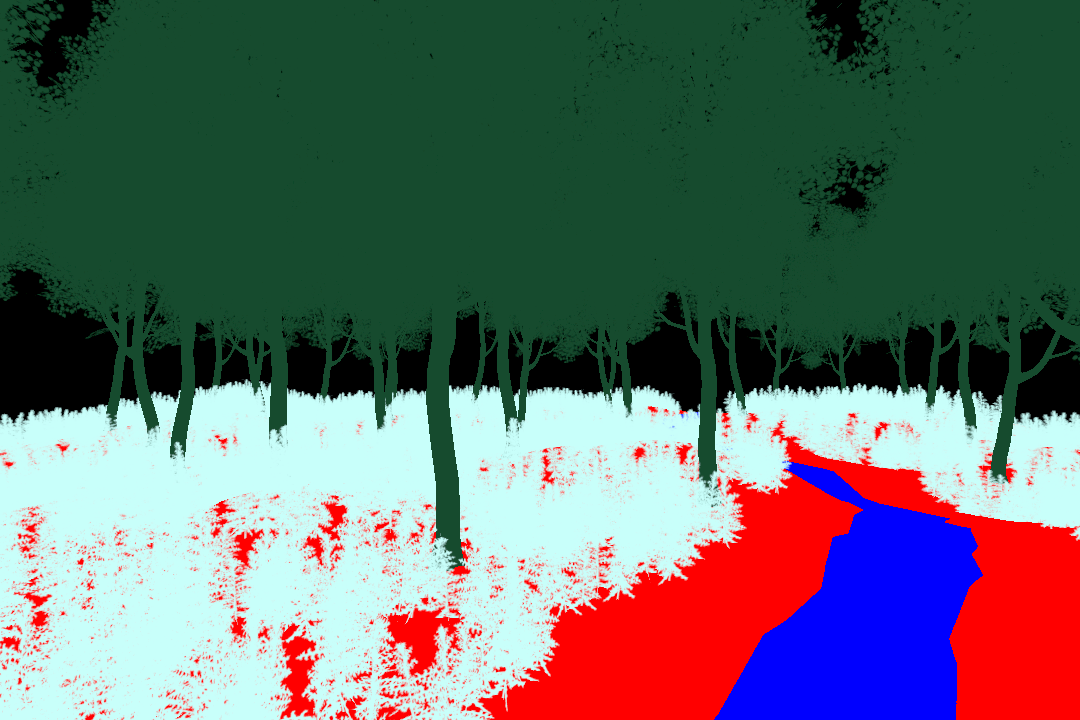
\includegraphics[width=\linewidth]{figures/validation/world_segmented.png}
    \end{subfigure}
    \hspace*{.5\linewidth}\begin{subfigure}{.5\textwidth}
        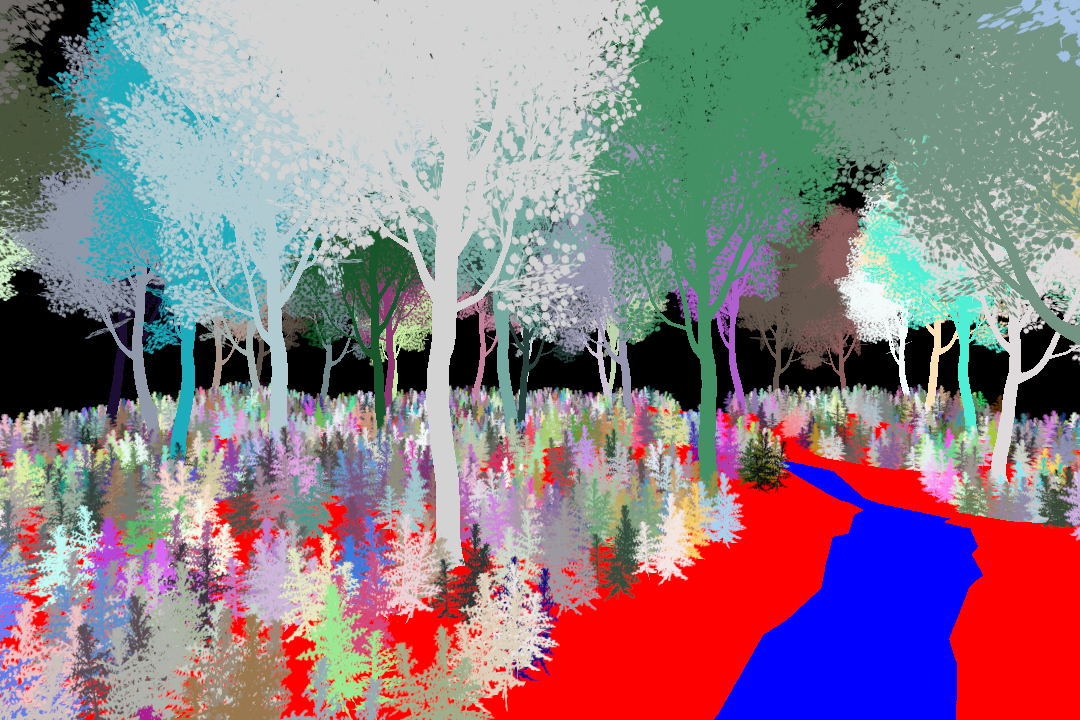
\includegraphics[width=\linewidth]{figures/validation/world_segmented_all.png}
    \end{subfigure}
    \caption{Example of object segmentation (up) and panoptic segmentation (down) on a generated terrain (left)}
    \label{fig:segmentation}
\end{figure}

% Introduce the task of object segmentation, and show how we use it to convert a regular image into a segmented image

\subsection{Presence and visibility of rivers} \todo{Show that this parameter can be used for estimation}
To show the visibility of the river in the landscape we analyse the proportion of the river in the terrain. As placement objects can obscure both a river and the terrain, this analysis is performed without the placement objects enabled.

To calculate the visibility of the river, the view of the camera is rendered with object segmentation, and from the pixels in the image the proportion of river against the entire terrain is calculated.

\subsubsection{Testing the visibility of rivers}
To test the visibility of the river, we take 500 samples of generated terrain, of which we calculate the percentage of terrain covered by the river. The result of this experiment is show in figure \ref{fig:river-visibility}. In these results, we see that the visibility of the river is very low, with more than 60\% of the samples being less than 5\%. One of the experiments where there is no river visible is shown in figure \ref{fig:river-visibility-results-low}. The generated terrain is shown in figure \ref{fig:river-visibility-results-low-world}. As seen, the generated river is very short, and only shown in the corner of the world. Because of this, it is not visible in the world. The world with the most visible river is shown in figure \ref{fig:river-visibility-results-high}. This river runs close to the camera, and therefore has a high visibility.

\begin{figure}
    \centering
    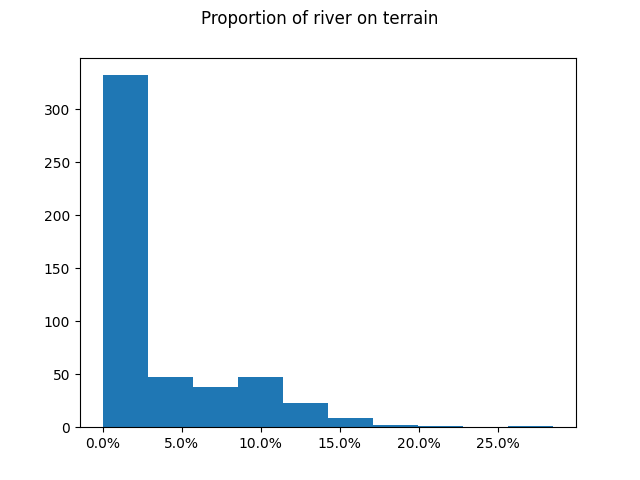
\includegraphics[width=0.8\linewidth]{figures/validation/2024-11-18_01-58-45_histogram.png}
    \caption{Histogram of the results of the river visibility test}
    \label{fig:river-visibility}
\end{figure}

\begin{figure}
    \begin{subfigure}{.5\textwidth}
        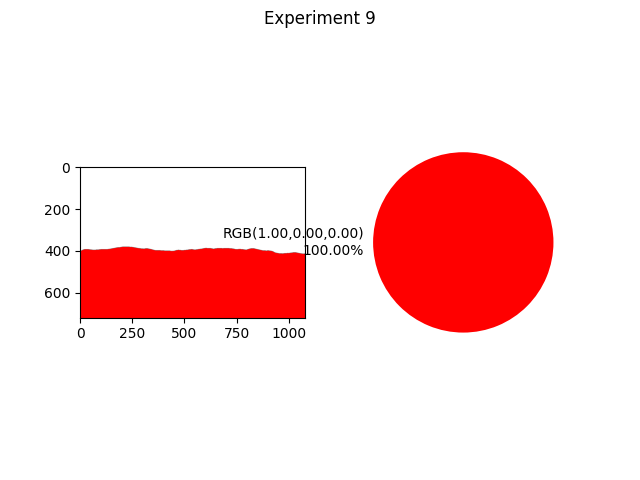
\includegraphics[width=\linewidth]{figures/validation/2024-11-18_01-58-45_9.png}
        \caption{Segmented view of a terrain without visible river}
        \label{fig:river-visibility-results-low}
    \end{subfigure}
    \begin{subfigure}{.5\textwidth}
        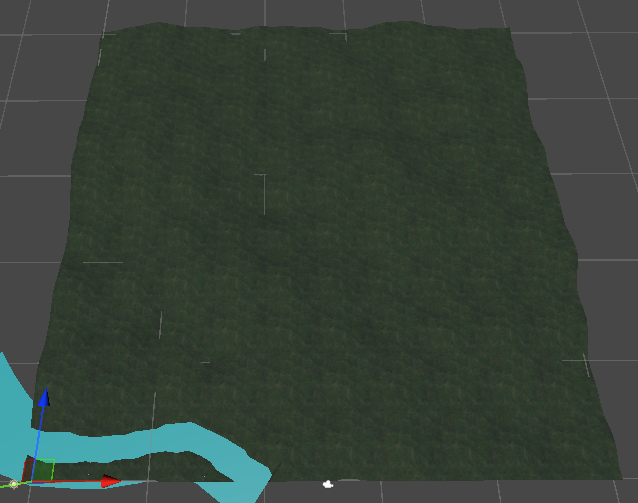
\includegraphics[width=\linewidth]{figures/validation/Bad river.png}
        \caption{Terrain of the view without a visible river}
        \label{fig:river-visibility-results-low-world}
    \end{subfigure}
    \begin{subfigure}{.5\textwidth}
        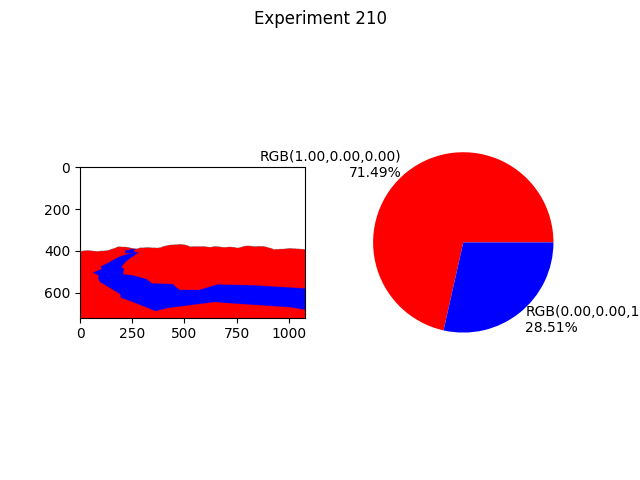
\includegraphics[width=\linewidth]{figures/validation/2024-11-18_01-58-45_210.png}
        \caption{Segmented view of terrain with the most visible river}
        \label{fig:river-visibility-results-high}
    \end{subfigure}
    \begin{subfigure}{.5\textwidth}
        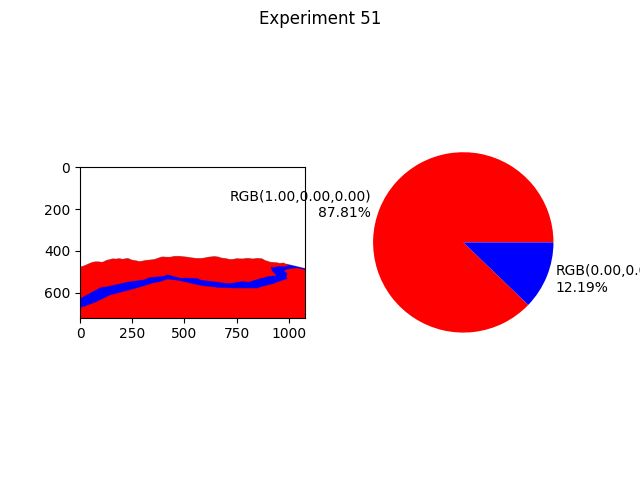
\includegraphics[width=\linewidth]{figures/validation/2024-11-18_01-58-45_51.png}
        \caption{Segmented view of terrain with medium visible river}
        \label{fig:river-visibility-results-medium}
    \end{subfigure}
    \label{fig:river-visibility-results}
\end{figure}

\subsubsection{Improving the visibility of rivers}
In the previous tests we kept the camera at a fixed position, namely on the centre of one side of the terrain. Instead of generating the terrain multiple times, the camera can be placed on any of the four sides of the terrain. This results in a different perspective on the terrain and therefore a different view on the river.

To test the improvement of this system, we perform the river visibility experiment, but for each terrain we calculate the visibility for each camera position, and take the camera position with the largest visibility. The histogram with the results of the experiments can be seen in figure \ref{fig:river-visibility-optimized}. From the results it shows that checking different camera positions does result in a terrain having a more visible river. Instead of more than 60\% of the experiments having no visible or nearly invisible river, selecting a different camera position has only 40\% of samples with a nearly invisible river. Although this method results in some terrains with a very large portion of water, with the largest proportion being 40\%, the largest increase in samples occurs between 10\% and 20\%.

\begin{figure}
    \centering
    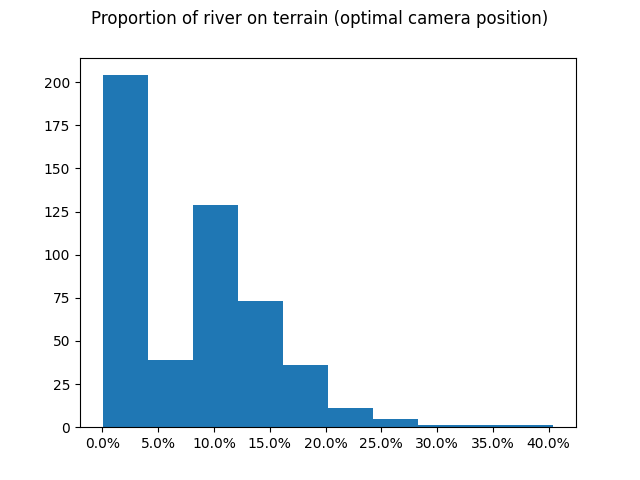
\includegraphics[width=0.8\linewidth]{figures/validation/2024-11-18_02-34-03_histogram.png}
    \caption{Histogram of the results of the river visibility test with the best camera position.}
    \label{fig:river-visibility-optimized}
\end{figure}


% Describe why we want to be able to see the rivers.
% Segmentation on terrain/water (not using placements)
% Show how we can find the proportion of surface that is river.
% Show examples of good/bad river representation.

\subsection{Single-object occlusion}



%\section{Discussion}
\todo{Intro?}

\subsection{Result of the terrain generation}
The system we have created is capable of generating digital landscapes containing rivers, smaller vegetation, and larger trees. The different components are connected to each other without overlapping, but they still create a visually solid environment.
In the environments created during testing, which represents a forested area, the generation terrain does not require large inclines, but it still results in a landscape that is not fully flat.
The generation of the river results in rivers that curve throughout the terrain, but the planning of the rivers does not work properly. Randomly placing points often results in rivers that generate mostly near the corners of the terrain and are not visible to the camera.
The placement of vegetation allows different types of plants to be placed on the terrain without overlap with each other or with rivers. The distribution can be configured to modify how plants spread or clutter in the environment.

The system is able to generate environments quickly enough. Running the testing setup, the system takes an average of 2.23 seconds to generate an environment with terrain, a single river, and vegetation. Further optimizations can improve this, but when only a small number of environments need to be generated, the current runtime is good enough.

%500 samples
%avg: 2.2303s
%stdev: 0.1332

% Discuss the architecture.
\subsection{Architecture}
In the architecture that we have defined, we have separated the different tasks of generating each terrain feature into one or multiple different components. Each of the components generates, transforms or combines parts of the system. Some of the components are separate to most others, such as the curve planner and fat curve generator, while others are used by a lot of different components, such as the cached intersections between fat curves and chunks.

The different components of the system can be divided into 3 categories, based on the different terrain features. The division of these categories is shown in figure \ref{fig:discussion-architecture-categories}. The first category, category A, is related to the generation of the terrain and the smallest category. Only the generation of the chunks is required to create the terrain. The second category, category B, is responsible for the planning and generating of the rivers, as well as combining the rivers onto the terrain. Category C is used to calculate the positions of objects to be placed onto the terrain using both the PDD and deformation field placement methods. This category depends on both categories, as it requires the heightmap of the chunks to place objects, and uses the rivers to filter object placements. In the figure, the intersections between fat curves and chunks are not divided into a category, since they are used for both category B and C.

% Todo: show why the categories make sense

\begin{figure}
    \centering
    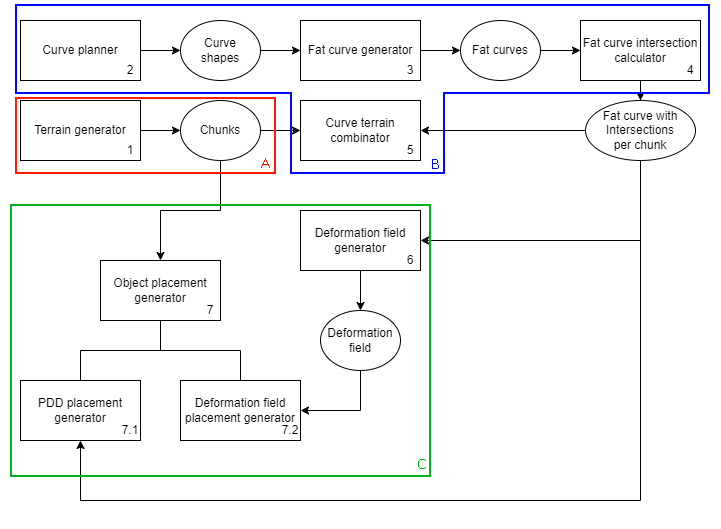
\includegraphics[width=\linewidth]{figures/architecture/Architecture-categories.png}
    \caption{Architecture of the system with components categorised for each environment feature}
    \label{fig:discussion-architecture-categories}
\end{figure}

% Discuss validation: PDD density
\subsection{Parameters of the system}
For each of the components in the system, we have established a set of parameters that influence the generated terrain. Some of these parameters, such as the size and resolution of the height maps of the terrain, can be kept constant for any generated terrain. With the other parameters, the user is able to influence the generated terrain. 
%A list of all parameters separated in these two categories can be found in appendix \ref{appendix:parameters}.

For the parameters related to the generation of the terrain, most of the parameters are very technical. The parameters of the fractal noise algorithm are mainly mathematical and are not accessible for users without experience with noise functions. Due to this, when a designer wants a specific feature on the terrain, more experimentation is required to generate a terrain that is acceptable to the user.

To plan the generation of the river, the parameters used have a clearer meaning to how they influence the system. The planned rivers follow a specific pattern, namely a meandering curve that can change directions randomly, and the parameters can influence the pattern the river takes. Differences to the amplitude of the meandering or the random rotation maximum can result in different characteristics of rivers, as shown in the research by Teoh \cite{teoh_riverland_2009}. In the current version of the system, there are no direct parameters that contribute to the initial position and direction of the river, so this is still a completely random process.
To transform the river path into a fat curve, the process mainly contains constant parameters. Since the interpolation of the path uses Bezier curves, a parameter has been added to derive the tangents of each control point. As this is mainly to control the smoothing of the curve, this parameter can be kept as a constant.

The parameters related to placing objects are closely related to the type of vegetation used. For the PDD algorithm, the parameters are related to the physical size of the objects that need to be placed. For trees, these are the outer radius which equates to the size of the canopy, which prevents overlap between trees, and the inner radius, which is to prevent overlap with smaller objects. In testing multiple layers of PDD placement have not beeen used, but the inner radius is still required for creating an initial deformation field for the second step of placing objects.

Before objects are placed using the deformation kernel method, the initial deformation field is generated. On this initial field the rivers and PDD objects are placed, to filter locations where plants cannot be placed. To allow for certain plants to be generated near or away of rivers, there are parameters that select the initial probability based on the fat curves. For PDD objects, the area within the inner radius of the PDD object is completely removed to avoid overlap between the two objects.

\todo{Deformation kernel itself}

\subsection{Validating system components}
To validate the generated terrain, we have used a number of different metrics to check and control the environment. Each of these methods analyses a specific component and how it affects the generated environment. Currently, these methods are not directly involved in the final terrain generation, but can instead be used after a terrain has been generated to improve the result.

% PDD density
For the placement of PDD objects, we have experimented with increasing the outer radius to reduce the density of trees. From this, we see an inverse relation between the radius of the object and the density of the objects within the area. To find this relation, we fitted two functions on the dataset, the exponential function and an inverse quadratic relation. These fits are shown in figure \ref{fig:discussion-pdd-graph}. For both fits, we calculated the mean squared error, which is shown in table \ref{tab:discussion-pdd-mse}. From this we can see that the quadratic relation has a better fit. This is expected, since increasing the radius linearly results in the area quadratically, which results in a quadratic decrease in the amount of points that can be placed. With this relation, the user has an indication of the expected density of the objects generated.

\begin{figure}
    \centering
    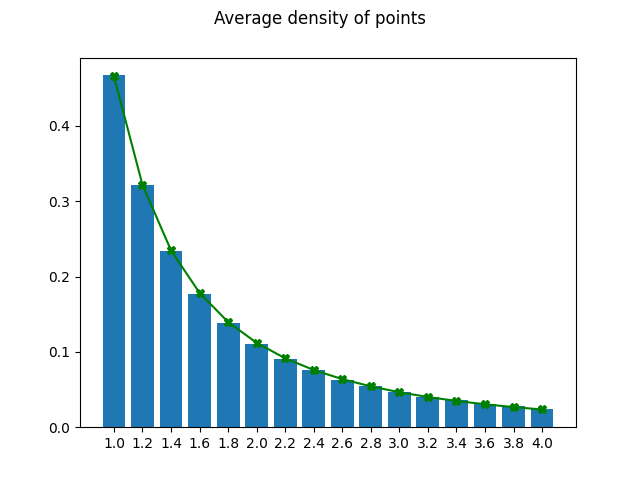
\includegraphics[width=0.5\linewidth]{figures/parameters/pdd-parameters-graph-fit.png}
    \caption{The density of points with varying ratios, with an exponential and inverse quadratic fit}
    \label{fig:discussion-pdd-graph}
\end{figure}

\begin{table}[h]
    \centering
    \begin{tabular}{|c|c|}
        \hline
        Function & MSE \\
        \hline
        Exponential & $3.97 * 10^{-5}$  \\
        Quadratic & $9.60 * 10^{-7}$ \\
        \hline
    \end{tabular}
    \caption{Mean squared error of different relations.}
    \label{tab:discussion-pdd-mse}
\end{table}

\subsubsection{River visibility}
In the current implementation of the system, generating a river that is visible is very unreliable. Since the start point and direction of the rivers are selected randomly, rivers often only traverses for a small distance before moving out of bounds or travels near a border that is not visible from the perspective of the camera. In the initial version more than 80\% of all rivers has a visibility of lower than 5\% of the total terrain surface, which results in a large number of terrains to be generated before an acceptable terrain appears. Improving this method by taking multiple camera positions into account has improved the system somewhat, although there is still a large proportion of all generated rivers that still does not contain a large section of the river. If a river is generated near the corner of the terrain, none of the camera positions will be able to view the river.

\subsubsection{Single object occlusion}
To validate whether the view is obscured by a large single object, we have used panoptic segmentation to calculate the size of each object in the view. With this, we found that the system sometimes generates objects close to the camera that take up almost all space in the view (Figure \ref{fig:single-object-large}).

The solution to remove all objects close to the camera has resulted in removing most large objects in the view. A few examples of terrains generated using this method are shown in Figure \ref{fig:discussion-tree-visibility-improved-examples}. Although the second rounds of experiments still contained objects that cover more than 30\% of the view, the large majority of views do not contain a large object in front of the camera. Although this approach seems to work well when looking at the statistics, the types of environment generated do look more sparse due to the empty space between the camera and the first trees. When generating a more dense environment, this approach removes a large part of this density.

\begin{figure}
    \begin{subfigure}{.5\textwidth}
        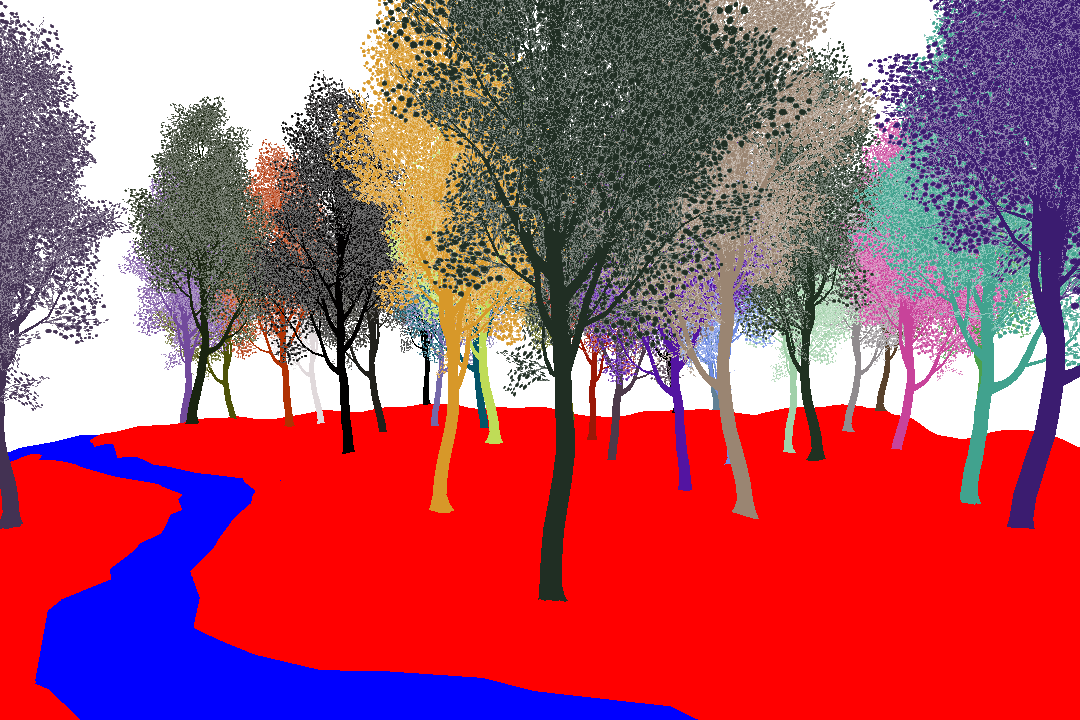
\includegraphics[width=\linewidth]{figures/validation/tree-visibility-improved-1.png}
    \end{subfigure}
    \begin{subfigure}{.5\textwidth}
        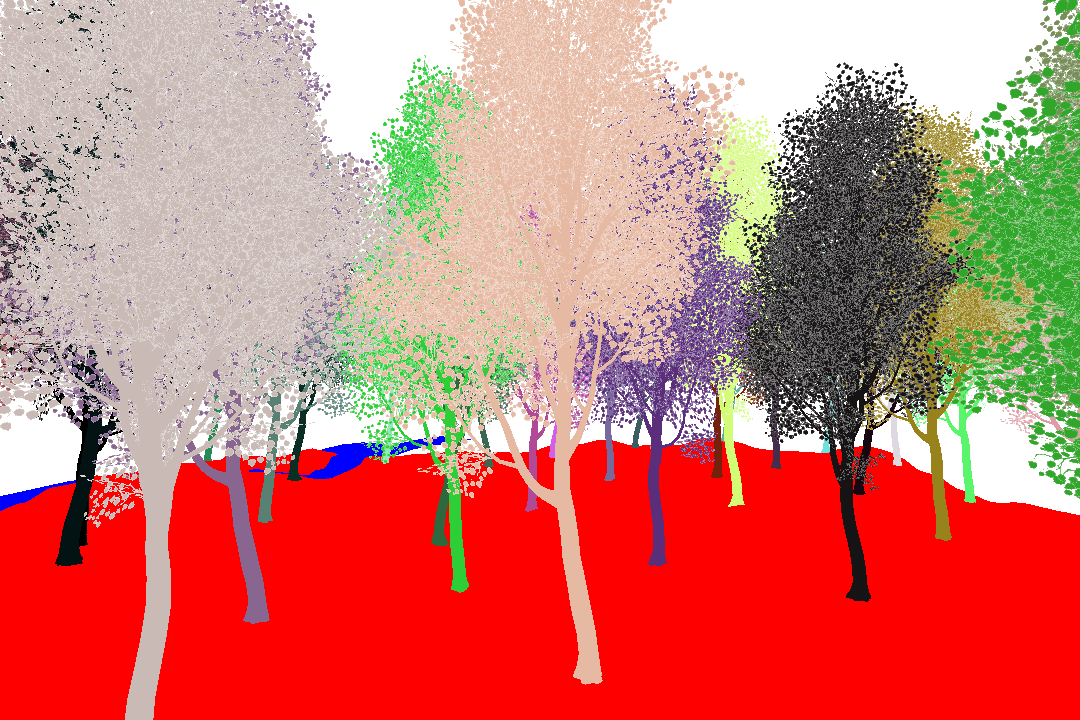
\includegraphics[width=\linewidth]{figures/validation/tree-visibility-improved-2.png}
    \end{subfigure}
    \caption{Examples of environments generated with objects closer than 11 units removed}
    \label{fig:discussion-tree-visibility-improved-examples}
\end{figure}


%\section{Future work}
In its current state, the system is able to generate environments containing vegetation and rivers, which can be manipulated using a set of parameters. However, there are still some improvements which can be made to the system to improve the features and capabilities of the system. A few of these improvements are described in the following section.

\subsection{Improving performance}
In the initial version of the system, there has been no focus on improving the performance of the system. One improvement that has been made is caching the intersection between fat curve triangles and chunks, but the performance of the system can be further improved by taking advantage of Unity's systems. One example would be to use parallelisation and SIMD by using Unity's job system in generating the terrain or operations with fat curves. A paper by Wei \cite{wei_parallel_2008} proposed a way to parallelise the Poison Disk Distribution, which can be applied to the object placement.

Although the current system is still able to generate landscapes in a reasonable time, shorter execution times can allow the user to generate more terrains in the same timespan, allowing for more choice in the resulting environment. \todo{More reasons?}

\subsection{Multiple environments}
While the system is able to generate environments with multiple types of vegetation, is not able to generate terrains with multiple types of environments. For example, the system cannot generate the edge of forests where a section of the terrain contains trees and the other section only contains grass or bushes. Interesting environments often contain different types of landscape, so, therefore, the addition of multiple types of environment should be added. Some research has already gone into the generation of multiple ecotope. Hammes \cite{hammes_modeling_2001} uses terrain features such as the height and slope of the terrain to determine which ecotope the section of terrain belongs to. Based on the ecotope, different plants are selected for placement. \cite{do_nascimento_gpu-based_2018}  and \cite{van_muijden_gpu-based_2017} take a similar approach, but both use water as well as the terrain, such that rivers also influence the selected ecotype.

\subsection{Generating roads}
In digital nature research, the presence of artificial objects is a desired component of the system \cite{van_houwelingen-snippe_designing_2023}. Because of this, one of the next features that should be added is the presence of roads or road networks. Roads can be planned on the terrain, and the addition will change the architecture. The planning and generation of roads has been researched before, most times in the procedural generation of cityscapes \cite{kelly_citygen_nodate} or in the procedural generation system by Smelik \cite{smelik_declarative_2011}. In addition to the placement of the roads itself, certain objects can be placed adjacent to roads, such as roads, sign posts or bins.

\subsection{Generating from point of view}
Although the aim of the system is to generate an environment for a single point of view, the generation techniques used are the same that are used to create large-scale environments. New techniques that involve the position of the camera more directly to generate each component can generate the environment more effectively. As mentioned in the discussion, rivers are not likely to be generated visible to the camera. When the position of the camera is taken into account, rivers can be generated such that they will appear in a certain position of the view. Additionally, the generation of objects can be changed by including the position of the camera to distinguish between foreground and background objects, which can result in interesting environments.


%\section{Conclusion}


\subsection{RQ 1: Terrain generation}
The system we have created currently supports 3 features: The surface terrain is generated using Fractal Perlin noise as a two-dimensional heightmap, and split into separate chunks. For each height map, a mesh is generated. This method is able to generate simple terrain with some ruggedness, which is enough for simple environments, such as forests.

To generate rivers, we randomly plan the path of a meandering river, which randomly turns at each step of the river planning. This path is transformed into a fat curve which is used in other steps of the program. Using the cross section of the river, the fat curve modifies the height map of the terrain to imprint the river bed and creates a mesh that represents the river surface. Although the generation of the river itself works, the river planning is very simplistic and often generates rivers that are not visible from the camera's perspective. From our experiments more than half of the terrains we have generated does not include a significant portion of the river in the view.

For the generation of vegetation we have selected two methods. The first method randomly places objects on a Poisson Disk Distribution, where all objects have a minimum distance where no other object can appear. With the other approach, a probability distribution is used to randomly place objects with each object modifying the distribution. Using different kernels changes the behaviour of objects placed, where certain kernels produce a prohibiting effect for other objects, while other kernels can attract objects to clutter near each other. Using both types of generation, different types of behaviour can be produced when generating the environment. To prevent overlap with rivers, the fat curve of the river acts as a filter for PDD objects, where objects are not generated if they are placed on a river. For the deformation kernels, the fat curve modifies the initial probability distribution to change the probability of an object placed on a certain part of the river. To place the objects onto the terrain, the height map is used to find the vertical position of the object on the terrain and the update is placed on the surface.

\subsection{RQ 2: Parameters of the system}
In the architecture we have created, each of the different components has a number of parameters that influence the generation or transformation of the specific feature. These parameters are categorised into two categories, where parameters can be considered as constant in most of the generated terrains, and parameters that change the terrain in order to get a desired effect.

For generating the terrain, most parameters are connected to the mathematical noise functions, and the influence of those parameters requires knowledge of these noise functions. The generation of rivers has parameters that describe the general shape and direction of the river. For the generation of objects, the parameters are inherent to the objects to be placed on the terrain. In the Poisson Disk Distribution, objects specify separate radii for objects of the same type or objects in a lower layer. In the deformation field, the objects placed specify how the probability field is modified in an area around the object. The amount of objects placed using the PDD is limited by the bounds of the terrain and the minimum distance, while the deformation uses a parameter to control the amount of objects generated.

\subsection{RQ 3: Validating terrain}
To validate the generated environments, we have selected three qualities of the terrain. For the first metric, we analyse the density of the generated trees. With the PDD algorithm, a minimum distance between each object is ensured, but by increasing this minimum distance, the density of objects decreases. This relation is an inverse quadratic relation and can allow the designer to estimate a density of objects the PDD algorithm will generate. When a certain density of objects is required, it can be calculated back to a minimum radius and then validated when the terrain is generated by counting each object.

For the second quality, the visibility of the generated rivers is analysed. In this metric, the generated terrain is evaluated by the proportion of river visible on the terrain. This method only analyses the surface, and therefore placed objects are removed. From this terrain object segmentation is used to calculate the amount of pixels that are either river or terrain. From this a ratio is calculated between the surface and the rivers, that can be used by a designer to find an acceptable range where a terrain contains enough visible river. When using multiple camera positions, such as each side of the terrain as is used as a method to improve the visibility of rivers, the same terrain can be used in some cases to provide a better view of the river, although this is not the case for all terrains.

For the placement objects, we analysed the visibility of each object, and looked at whether some objects take up a significant portion of the screen. Instead of object segmentation, panoptic segmentation is used where each individial object is separated. For each terrain, the pixels per objects are counted and calculated as the proportion of the total screen size. From this we have seen that some objects occupy a significant portion of the screen. With these proportions, large objects can be removed if they block a large part of the view, or find a minimum distance where most large objects appear in and remove all objects within this distance.
 % Possibly merge futurework/conclusion

% discussion

% future work

\bibliographystyle{plain} % We choose the "plain" reference style
\bibliography{references} % Entries are in the refs.bib file

\end{document}
